\documentclass[11pt,letterpaper]{article}

\usepackage{graphicx}
\usepackage[margin=1in]{geometry}
\usepackage{amsmath}
\usepackage[T1]{fontenc}
\usepackage[utf8]{inputenc}
\usepackage{authblk}
\usepackage{fancyhdr}
\usepackage{lastpage}
\usepackage[parfill]{parskip}
\usepackage{subcaption}

\pagestyle{fancyplain}
\fancyhf{}
\fancyfoot[R]{\footnotesize Page \thepage\ of \pageref{LastPage}}

\renewcommand{\headrulewidth}{0.0pt} % No header rule
\renewcommand{\footrulewidth}{0.4pt} % Thin footer rule

\begin{document}

\title{Visual Discovery of Communication Patterns in Email Networks}

\author[ ]{Benjamin Bengfort}
\author[ ]{Konstantinos Xirogiannopoulos}
\affil[ ]{Department of Computer Science}
\affil[ ]{University of Maryland}
\affil[ ]{\textit{\{bengfort,kostasx\}@cs.umd.edu}}

\date{April 6, 2015}

\maketitle

\section*{Introduction}

In the age of social networks, it is very popular to analyze Twitter and Facebook to detect relationships and communities and to discover how information flows between groups. However, both Facebook and Twitter are examples of ``performed'' social networks: because a user has full control over who he or she ``friends'' or ``follows,'' he can artificially create a persona that he wishes the outside world to perceive him as. In fact, it has been well-studied that expressions of taste typically exclude the most critical groups to communication flows, and that social networks are merely the expressions of performed taste \cite{liu_social_2007}.

Email, on the other hand, is used in every facet of modern life and typically includes and aggregates facets of ourselves that would otherwise be segregated -- for example, professional and personal personas. Because we spend so much time writing, reading, and responding to email, it has become integrated into a communication fabric that far exceeds other media that may get more analytical attention like text messaging or social networks. Email, therefore, can be seen to embed a natural communication network, from which we can extract rich insights about actual communications and influences within a single ego network -- the email inbox of a single user -- without the bias of taste performance.

%If a user could be equipped with some understanding of the natural communication flow in a non-performed communication domain, we believe it would lead to more effective communication.
In this paper, we will explore the visual analysis of two personal email networks, one from each of the authors, where one network is extremely large in terms of the number of nodes (email addresses) and the other network is extremely large in terms of the number of edges (cliquish, highly-connected email). We hope to show that if a user can visualize their own networks, they will better understand the dynamic nature of their communication in terms of key players, communities, and gaps in communication. Through such visual understanding, users may be better able to respond to, and manage the constant flow of email messages in a meaningful way.

We will use Gephi \cite{gephi_gephi-open_2010} to visualize email networks that have been extracted from \texttt{mbox} files via a Python tool written by the authors called \texttt{tribe}, which serializes the network into GraphML \cite{brandes_graph_2010}. Gephi has been used for visual exploration and mapping of networks \cite{bastian_gephi:_2009} and includes many features for the statistical analysis of small to medium networks \cite{mcsweeney_gephi_2009}. Work of note demonstrates the analysis of dynamic network connections within Twitter conversations \cite{bruns_how_2012}, which shows how Gephi might be used for dynamic networks whose topology can rapidly shift, as in email. As part of our analysis we will critique Gephi and provide a contrast to NodeXL \cite{smith_nodexl:_2010}, another popular tool for visual network analysis.

\subsection*{Using Email as a Dataset}

Email networks are often extremely complex, involving many actors and communication channels. A single user may have multiple email addresses, requiring some form of entity resolution to aggregate nodes into a single canonical person. Semantic preference might arise in the inclusion of participants in an email conversation, for example; inclusion in a CC rather than in the TO field of an email indicates that one might be solely a witness to conversation, not an actual participant. These challenges, coupled with the fact that email is extremely personal and private, has made it more difficult to explore the networks that exist in email data, while the public nature of social networks often leads researchers to explore that domain more fully.

\begin{figure}[h]
	\centering
	\begin{subfigure}{0.49\textwidth}
		\centering
		
\includegraphics[width=\textwidth]{figures/benjamin_descriptive.png}
		\caption{\textsf{Benjamin Bengfort (large)}}
        \label{fig:benjamin_descriptive}
	\end{subfigure} \hfill
	\begin{subfigure}{0.49\textwidth}
		\centering
		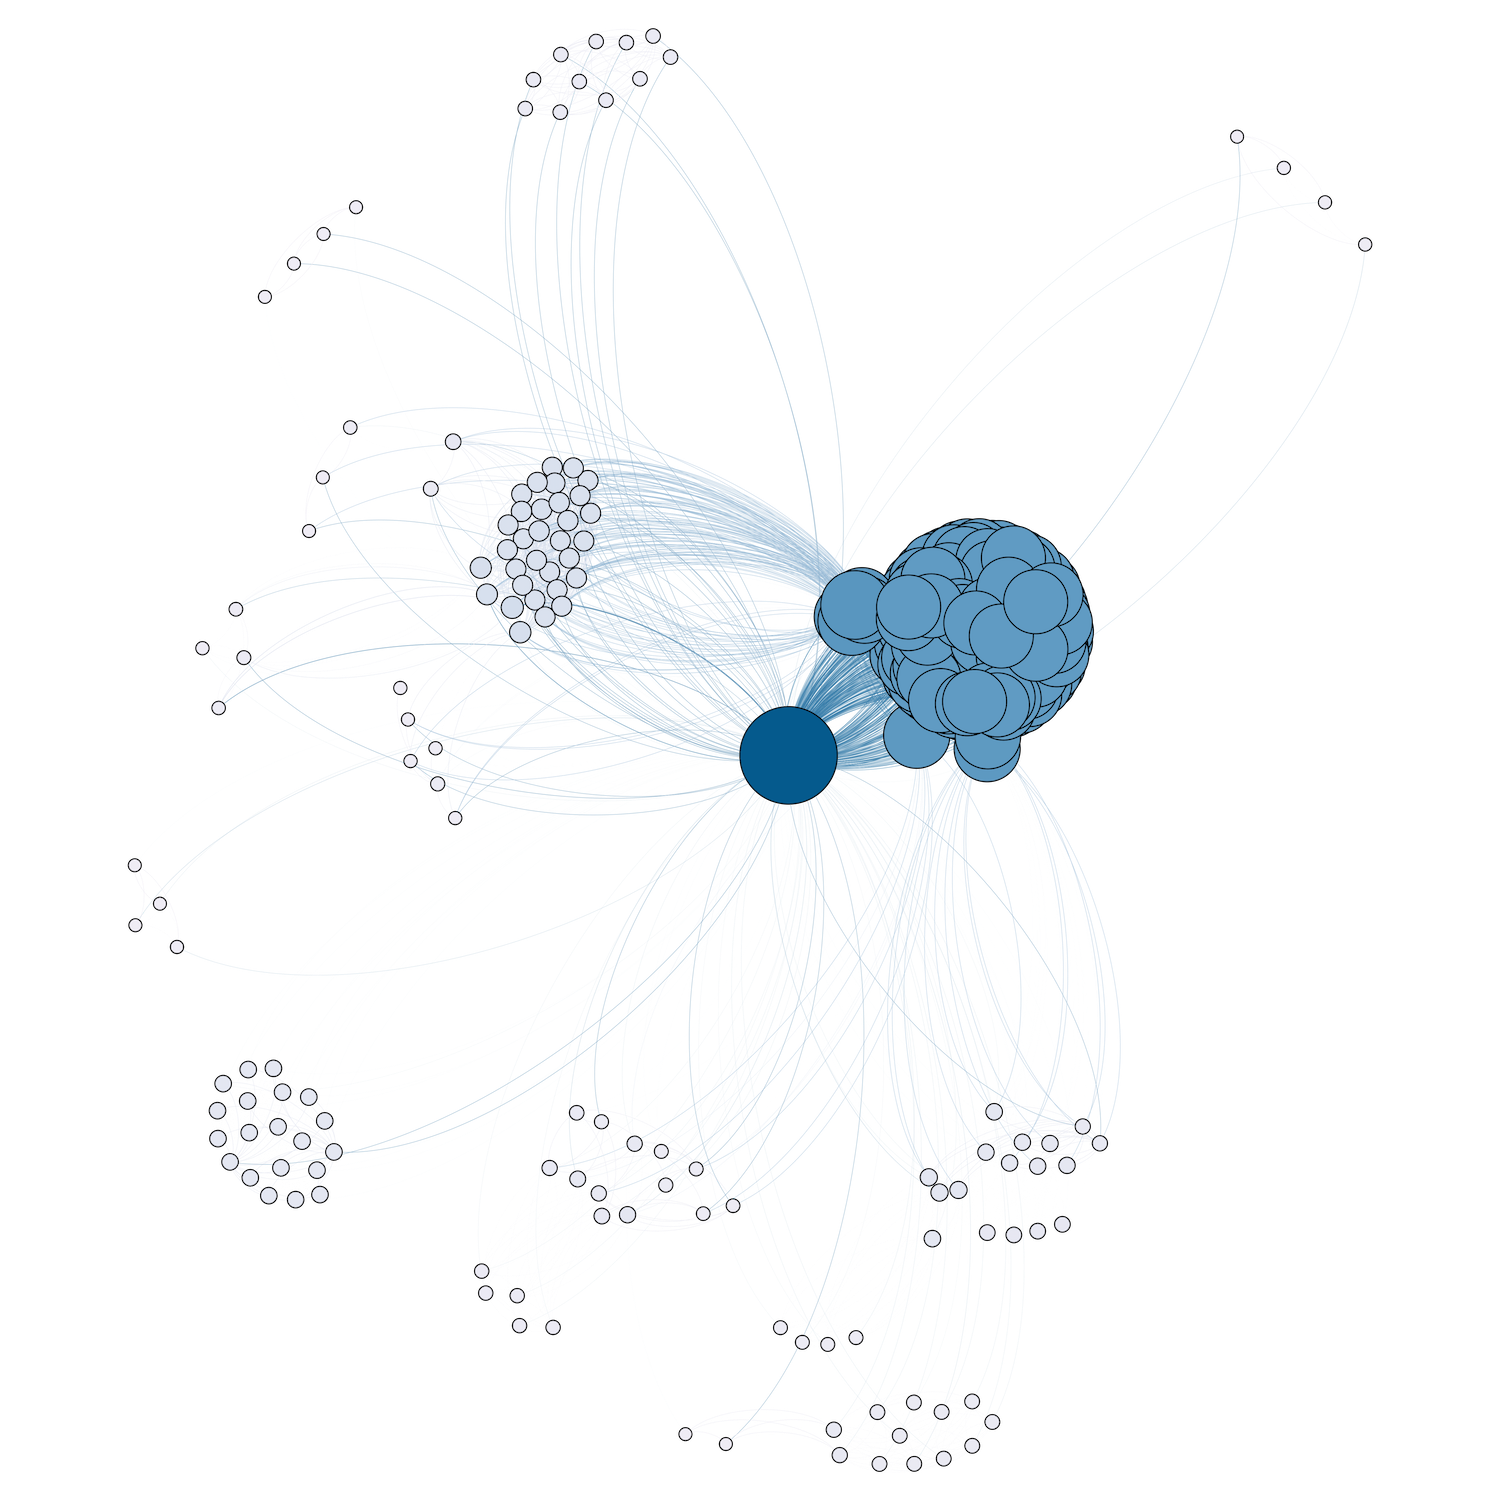
\includegraphics[width=\textwidth]{figures/kostas_descriptive.png}
		\caption{\textsf{Konstantinos Xirogiannopoulos (small)}}
        \label{fig:kostas_descriptive}
	\end{subfigure}
    \caption{\textsf{Email networks, no matter the size, are complex.}}
    \label{fig:descriptive}
\end{figure}

As shown in Figure \ref{fig:descriptive}, the authors have elected to use their personal email networks, and through a simple initial visualization it becomes clear that email networks are large and complex.  The nodes in these networks represent the unique email addresses of the individuals who are participating in email communications, and the edges indicate a relationship in one or more email messages, that is that both email addresses were included together in at least a single email in either the \texttt{FROM}, \texttt{TO}, or \texttt{CC} fields. Undirected edge weights on the graph indicate the frequency of communication that includes two email addresses: the more frequently two email addresses are together on the same email, the stronger the weight. Table \ref{tab:network_comparison} gives descriptive statistics on the relative sizes of these two networks.

\begin{table}[t!]
    \centering
    \begin{tabular}{l | c c}
        \hline
        Metric & Benjamin & Kostas \\
        \hline
        Emails & 52,716 & 9879 \\
        Nodes & 3,408 & 1,005 \\
        Edges & 37,158 & 56,370 \\
        Avg. Degree & 21.8063 & 112.1791 \\
        \hline
    \end{tabular}
    \caption{Description of Email Datasets}
    \label{tab:network_comparison}
\end{table}

Although these networks are comparable, because Benjamin's network has three times the number of nodes as Kostas' network, we have elected to call it the ``large'' network. Interestingly, Kostas' ``small'' network has significantly more edge connections, and is more connected than Benjamin's graph. We found that this had a very large impact on the choice of layout algorithm to use for the network visualizations. The ``large'' network responded very well to the Yifan Hu \cite{hu_efficient_2005} layout, which tended to elongate the network and spread nodes apart in clusters. On the other hand, the ``small'' network was more suitably laid out by the Fruchterman Reingold method \cite{fruchterman_graph_1991}. Note that neither of these relatively medium sized graphs responded well to the Gephi default layout, the Force Atlas 2 Continuous Layout \cite{jacomy_forceatlas2_2014}.

For the sake of comparison and diversity in our examples, we have extracted both of our email networks, and compared them through several statistical methods. These methods allows for more concrete and reliable analyses and demonstrate how network visualization can yield very important insights on vast and complex interconnected data. This is possible primarily because both email networks exhibit a power law degree distribution, which is common to social networks and indicates that many desirably properties exhibited by natural, human networks can be extracted. The power laws distribution visualization in Figure \ref{fig:degree} was created by Gephi, and is part of the suite of statistical and reporting tools Gephi is known for.

\begin{figure}[h]
	\centering
	\begin{subfigure}{0.49\textwidth}
		\centering
		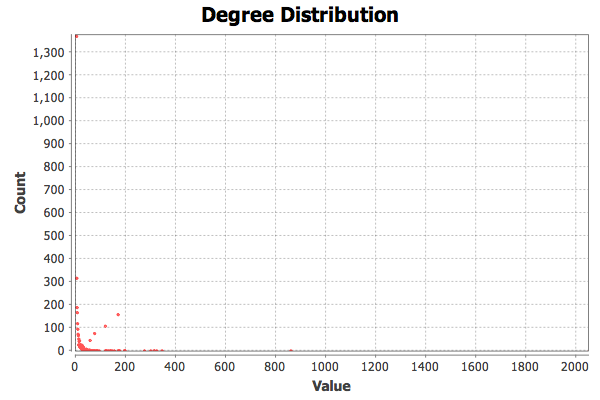
\includegraphics[width=\textwidth]{figures/benjamin_degree.png}
		\caption{\textsf{Benjamin Bengfort (large)}}
        \label{fig:benjamin_degree}
	\end{subfigure} \hfill
	\begin{subfigure}{0.49\textwidth}
		\centering
		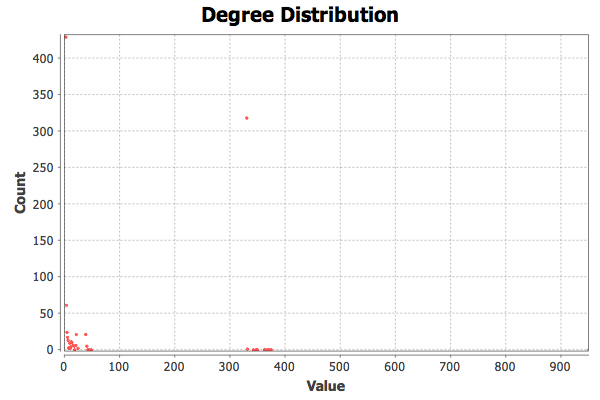
\includegraphics[width=\textwidth]{figures/kostas_degree.png}
		\caption{\textsf{Konstantinos Xirogiannopoulos (small)}}
        \label{fig:kostas_degree}
	\end{subfigure}
    \caption{\textsf{Degree distribution follows a power-laws distribution, common to natural social networks.}}
    \label{fig:degree}
\end{figure}

\subsection*{Data Wrangling for Gephi}

Unlike NodeXL, Gephi does not have native graph extraction tools for social media. While it does include an email extraction tool, we were unable to get it to function correctly. We instead decided to rely on a tool created by the authors called \texttt{tribe}, which is freely available as an open source project at \textit{https://github.com/districtdatalabs/tribe}. The process for extracting a graph from email deserves some attention, as it affects the way that these email networks are visualized. First, the email \texttt{mobx} had to be exported from Gmail using Google's data export tools. The \texttt{tribe} scripts were then used to extract the graph as follows:

\begin{enumerate}
    \item For every email, collect all email addresses from the \texttt{TO}, \texttt{CC}, and \texttt{FROM} fields.
    \item Find all combinations of email address and create an edge for each pair, where the email addresses are lexicographically sorted.
    \item Count the number of unique email pairs, and the total number of edges in the network.
    \item Assign edge weights for each email pair based on its frequency relative to the size of the network.
\end{enumerate}

The \texttt{tribe} tool exported the graph to disk using the GraphML file format, which is easily importable into Gephi. The GraphML implements a property graph data structure, and therefore is able to embed additional information than simple adjacency lists; for example the domain of the email and domain frequency. Although these tools weren't used in this particular analysis, it's worth nothing that we had to combine a third-party tool with Gephi in order to have as complete a framework as NodeXL. Even though Gehpi does have a ``data laboratory'' similar to a spreadsheet, import and export via GraphML was by far the easiest workflow for us.

\section*{Insights}

% Kostas: Since we have a separate section for the headlines, I don't think this section is necessary. We just talk about the insights in every headline...

% Ben: you're probably right, but an intro paragraph here will not make it look bad, and also the subsection is smaller font, which is better for longer headlines. I leave it up to you, but I think this structure is good.

We intended our analysis of the large and small email networks to demonstrate the discovery of central players, communities, and critical communication channels in a visual manner. We explored three primary techniques for visualization: motif simplification to reduce the complexity of the graph, centrality visualization to identify key players or information channels, and clustering mechanisms to discover communities. The exact same analyses (or steps) were performed on each email network in sequence, although some minor adjustments were made in layout and formatting to deal with anomalies or peculiarities in individual data sets. For the most part, the visualizations shown and described in this section can be compared side-by-side as having had the same methodology applied to each.

\subsection*{Motif Simplification Reveals Surprising Hubs of Information Flow}

\begin{figure}[h]
	\centering
	\begin{subfigure}{0.49\textwidth}
		\centering
		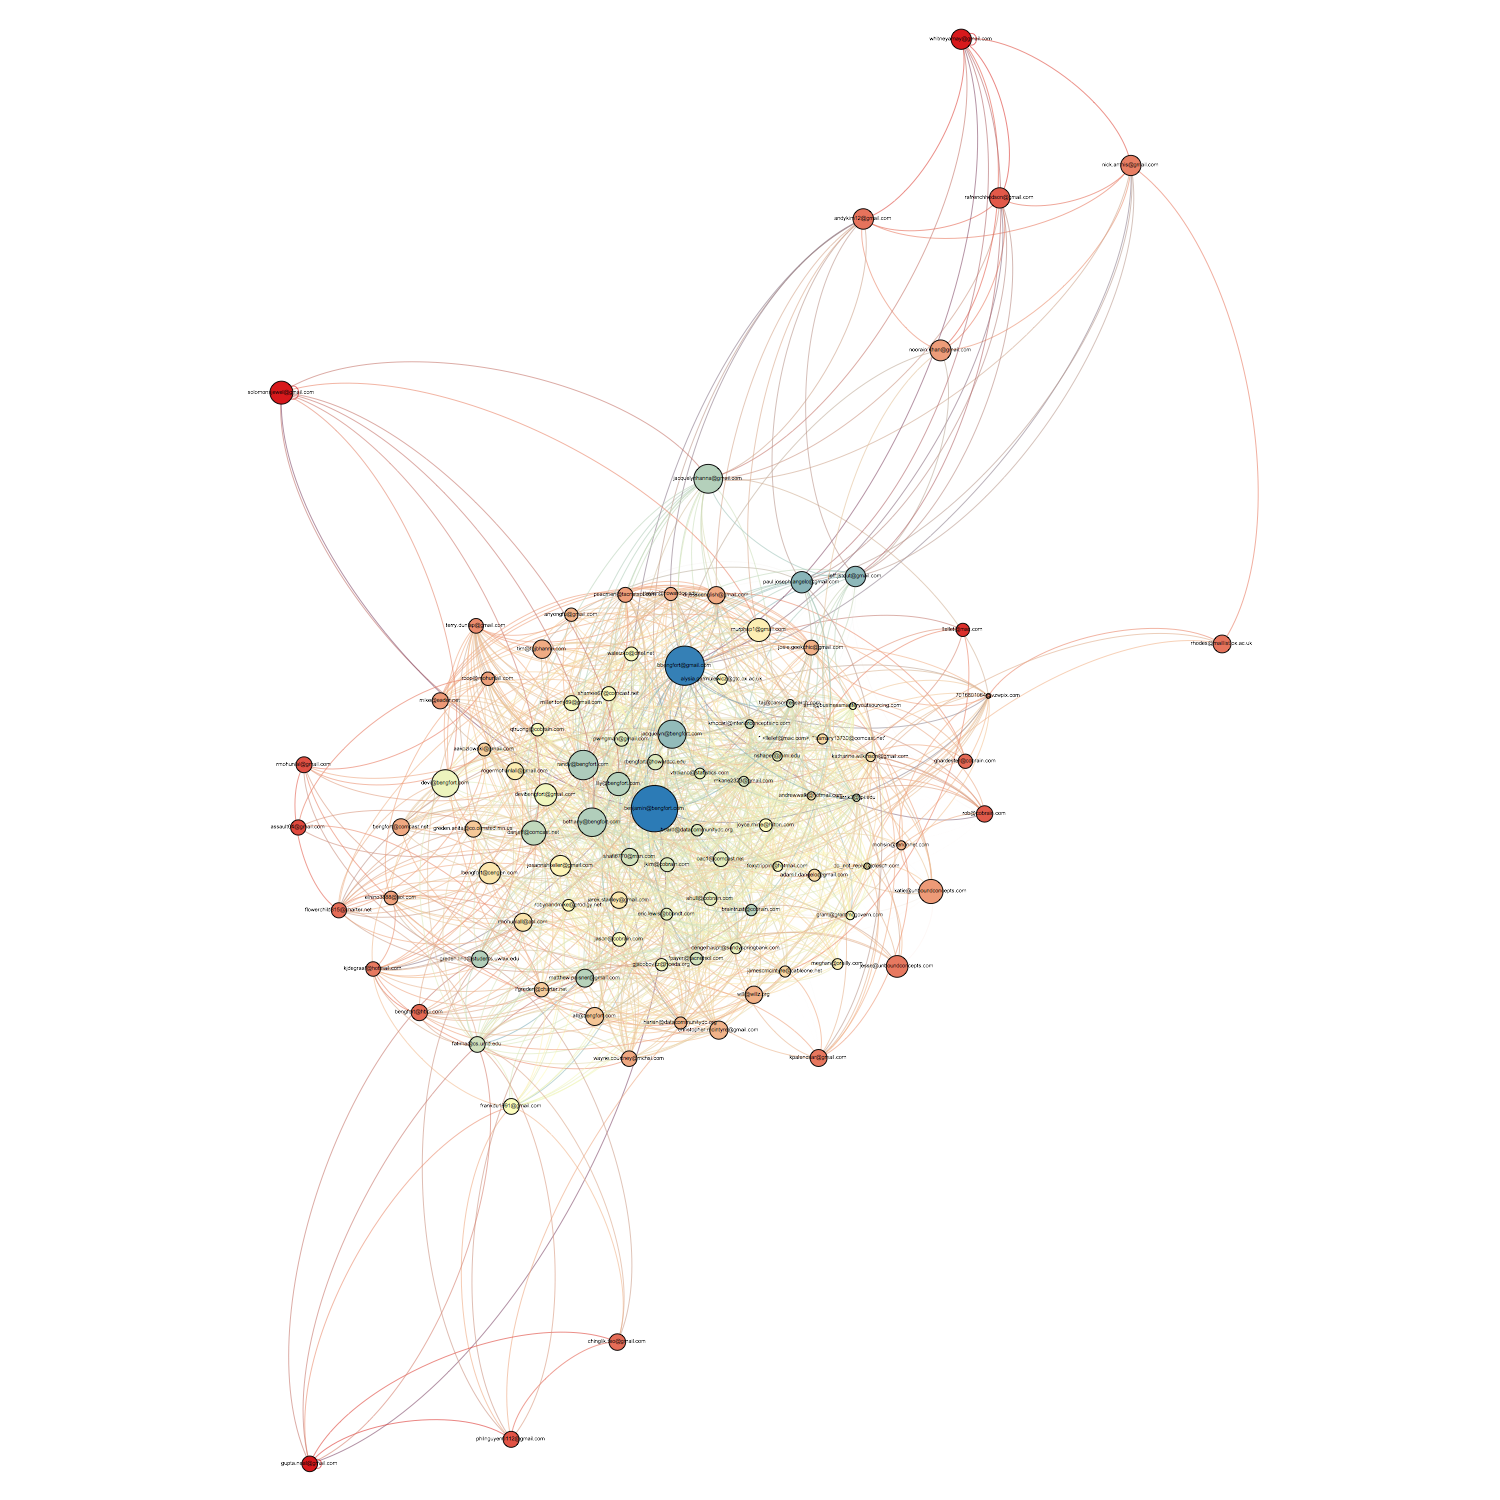
\includegraphics[width=\textwidth]{figures/benjamin_simplification.png}
		\caption{\textsf{Benjamin Bengfort (large)}}
        \label{fig:benjamin_simplification}
	\end{subfigure} \hfill
	\begin{subfigure}{0.49\textwidth}
		\centering
		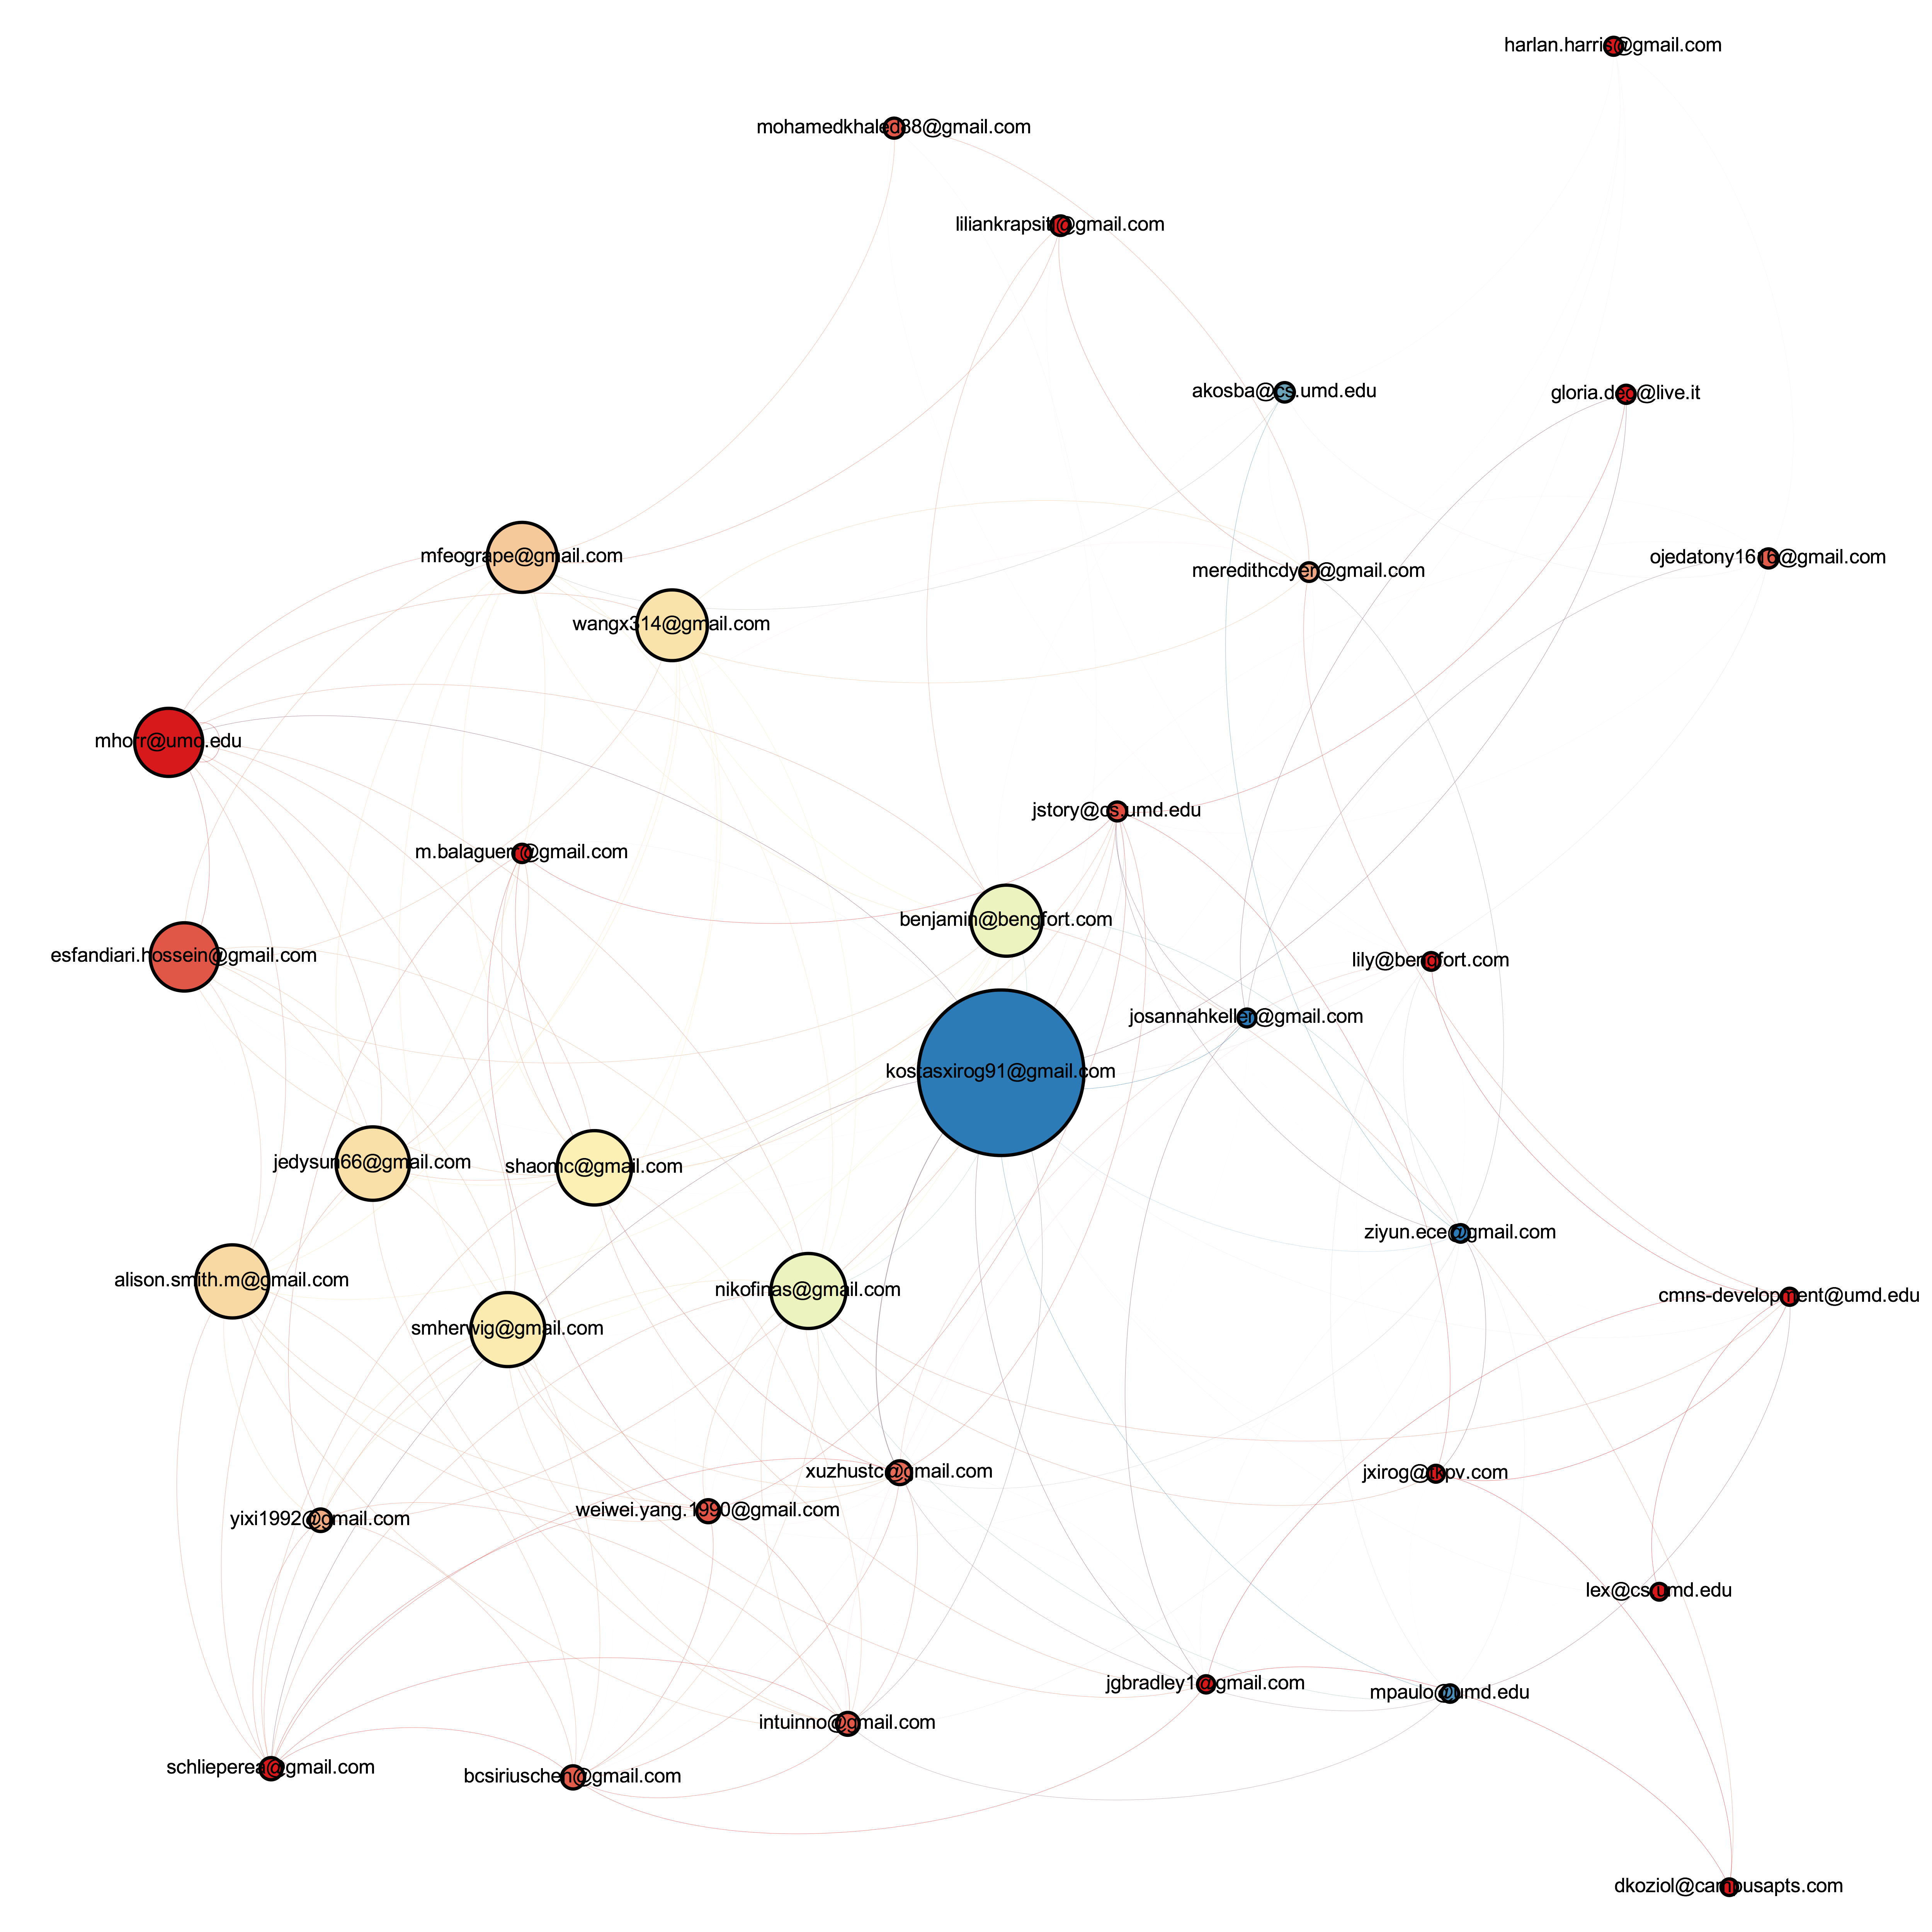
\includegraphics[width=\textwidth]{figures/kostas_simplification.png}
		\caption{\textsf{Konstantinos Xirogiannopoulos (small)}}
        \label{fig:kostas_simplification}
	\end{subfigure}
    \caption{\textsf{Grouping by ``Hub'' reveals a simpler graph with interesting communication flows.}}
    \label{fig:simplification}
\end{figure}

Unfortunately, Gephi does not have the same suite of tools for motif simplification that NodeXL does. Within the Gephi visualization process you can adjust the size, shape, and color of nodes and their labels as well as the color of edges. In order to demonstrate network simplification analyses similar to ``fans'' and ``connectors'' in NodeXL, we instead used a grouping technique to combine similar or highly connected nodes into a single node thus reducing the number of nodes in the network. We also hoped to utilize a force-directed edge bundling technique to simplify the edge visualization, a feature reported to be in Gephi \cite{pupyrev_edge_2012,gansner_multilevel_2011}, but unfortunately was unavailable in the current stable version. Figure \ref{fig:simplification} shows how the grouping process can immediately alleviate the complexity of the graph and quickly indicate the most critical hubs of information flow.

Our methodology to simplify the graph used Gephi ``deduplication'' based on the \texttt{HITS} computation of authority. This methodology computed the node with the highest number of one- and two-degree triangles within each geodesic, that is, which node is the most connected node in a two degree neighborhood that also participates in the shortest path. This technique reduced the ``large'' graph to 61 nodes and the ``small'' graph to only 29. Because these graphs were more visually manageable from a human understanding perspective, these are also the only graphs to which we were able to assign readable labels.

The reduction of nodes was also coupled visual motifs. The ``authority'' of each node was reflected by the size of the node. Furthermore, we used ``betweenness centrality'' to color the nodes on a continuous gradient scale, where red nodes have a smaller betweenness centrality and blue nodes a larger. Unfortunately it was impossible to include legends using Gephi, so they were necessarily omitted from the figures.

We were surprised when we reviewed the email addresses of the nodes that were selected as \textit{hubs} -- they were unexpected relative to the nodes that the authors might have selected. In both networks the large node in the center is the ego -- the email address of the author whose email inbox we are analyzing. The ego is surrounded by green and light blue colored nodes, indicating, medium centrality nodes that are critical to information flow in the network, these nodes are family, close friends, and colleagues as might be expected. However, around the periphery are light yellow and red colored nodes which act as hubs for more distant clusters of email addresses where email communication is occasional. The hubs in the outer layer are often not ones the authors associate with direct email communications, but rather are more often included or CC'd in email messages. This effect was observed for a variety of email conversations and domains (work, school, different sets of friends) where the nodes become more authoritative in the communication process between distinct clusters.

\subsection*{Central Nodes Don't Often Have a High Degree of Contacts}

\begin{figure}[h]
	\centering
	\begin{subfigure}{0.49\textwidth}
		\centering
		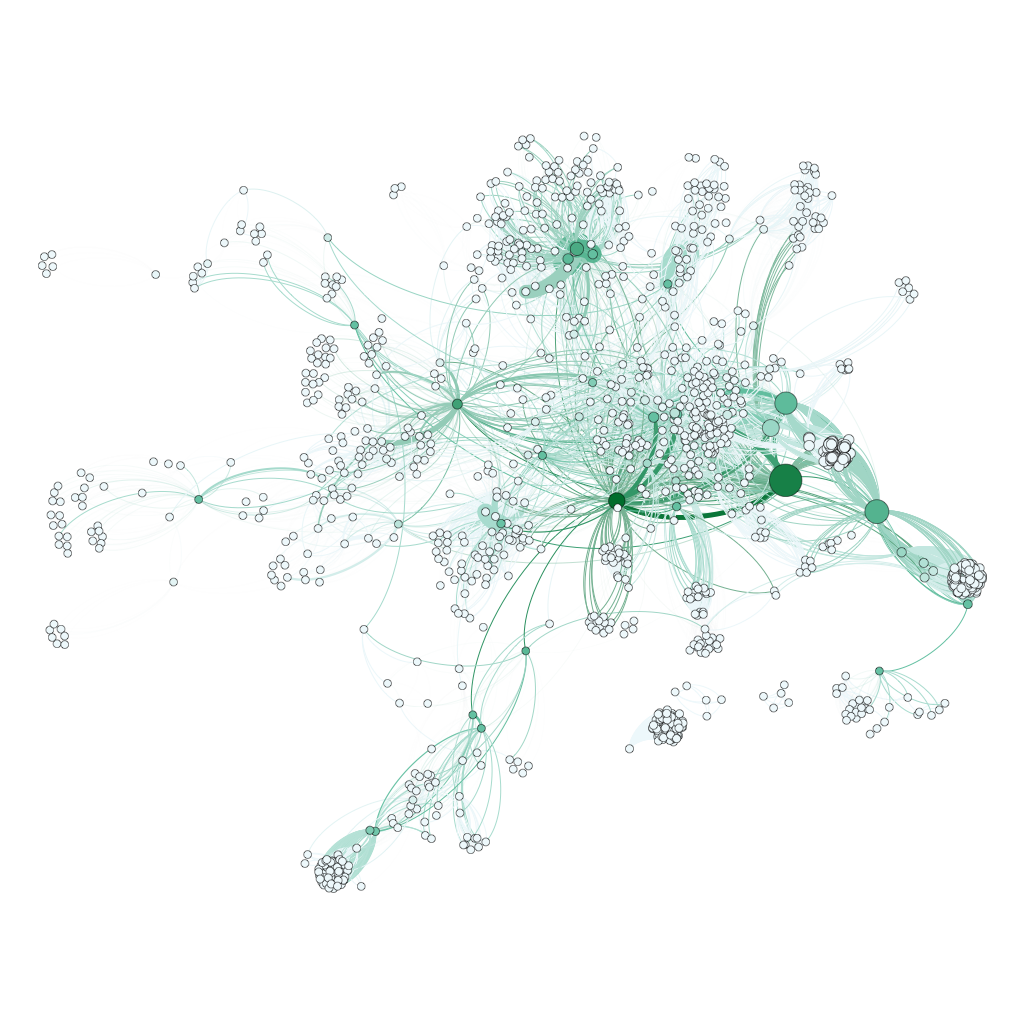
\includegraphics[width=\textwidth]{figures/benjamin_centrality.png}
		\caption{\textsf{Benjamin Bengfort (large)}}
        \label{fig:benjamin_centrality}
	\end{subfigure} \hfill
	\begin{subfigure}{0.49\textwidth}
		\centering
		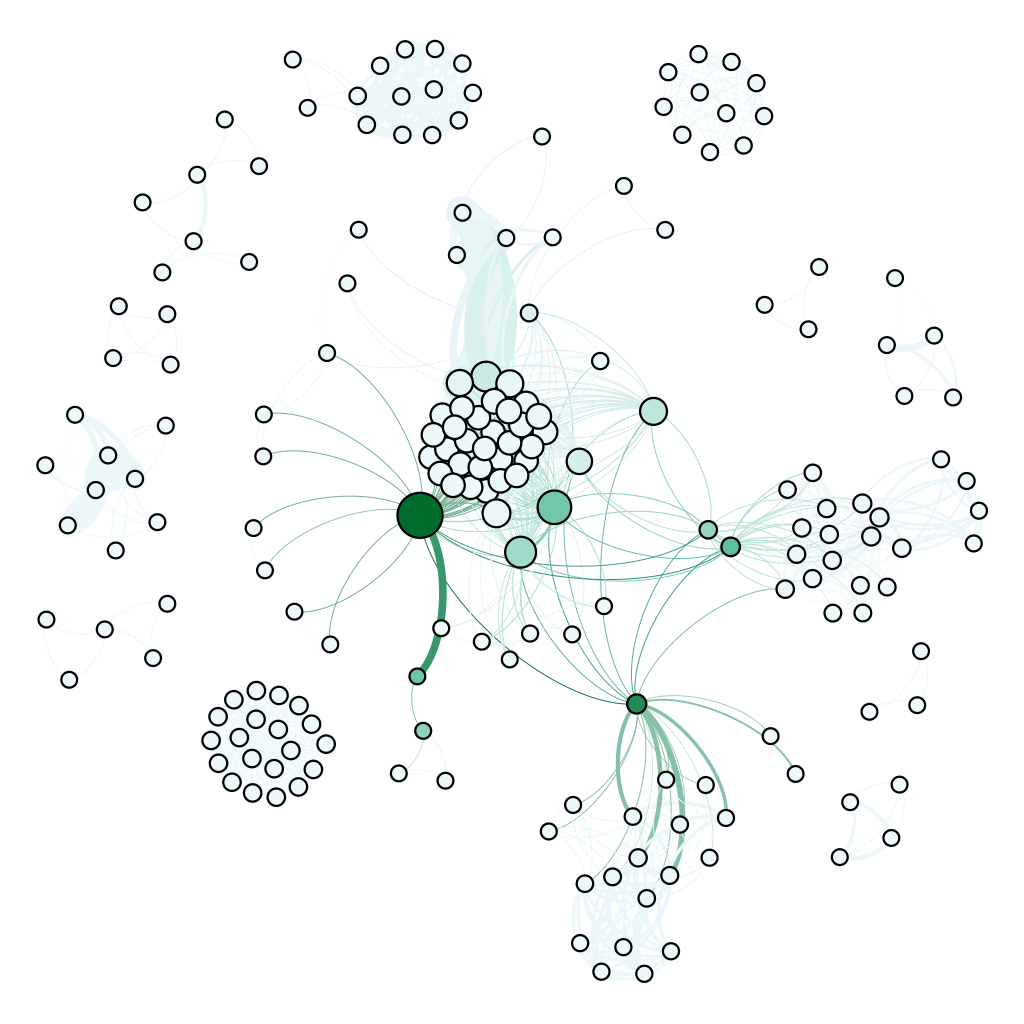
\includegraphics[width=\textwidth]{figures/kostas_centrality.png}
		\caption{\textsf{Konstantinos Xirogiannopoulos (small)}}
        \label{fig:kostas_centrality}
	\end{subfigure}
    \caption{\textsf{Nodes highlighted for their high betweenness centrality}}
    \label{fig:centrality}
\end{figure}

Our next exploration of critical communication channels followed from the idea that surprising nodes had authority because of their degree (the number of edges connected to a node). Instead, we wanted to include as many nodes as possible and measure their centrality to show important individual nodes in the flow of information across the network. In order to simplify the graph without losing too much information, we filtered nodes such that only nodes connected to the \textit{giant} (the email of the inbox) with a degree of 4 or more remained. This removed approximately 60\% of the nodes, but only 10\% of the edges. In order to better visualize key players, the ego node (also refered to as the giant in filtering) was removed from the visualization, as it was obviously the most central node in the network.

In Figure \ref{fig:centrality}, the green gradient scale represents the betweenness centrality of each node, where dark green is a high centrality score and white nodes are not central. The size of the node is related to degree centrality -- how many email contacts the node has in the network. This graph reveals that the nodes with a high betweenness centrality, who are members of many geodesics (shortest paths), are located in critical parts of the structure of the graph (by connecting disparate groups), but for the most part do not have a high degree. These ``connective'' nodes are usually actors who facilitate communication between one group and another, often directly through the ego node. It's a bit surprising that they don't always have a a high degree; instead each critical node seems to join specific, smaller subgroups rather than multiple larger groups.

\subsection*{Communication Load Varies Widely Between Communities}

\begin{figure}[h]
	\centering
	\begin{subfigure}{0.49\textwidth}
		\centering
		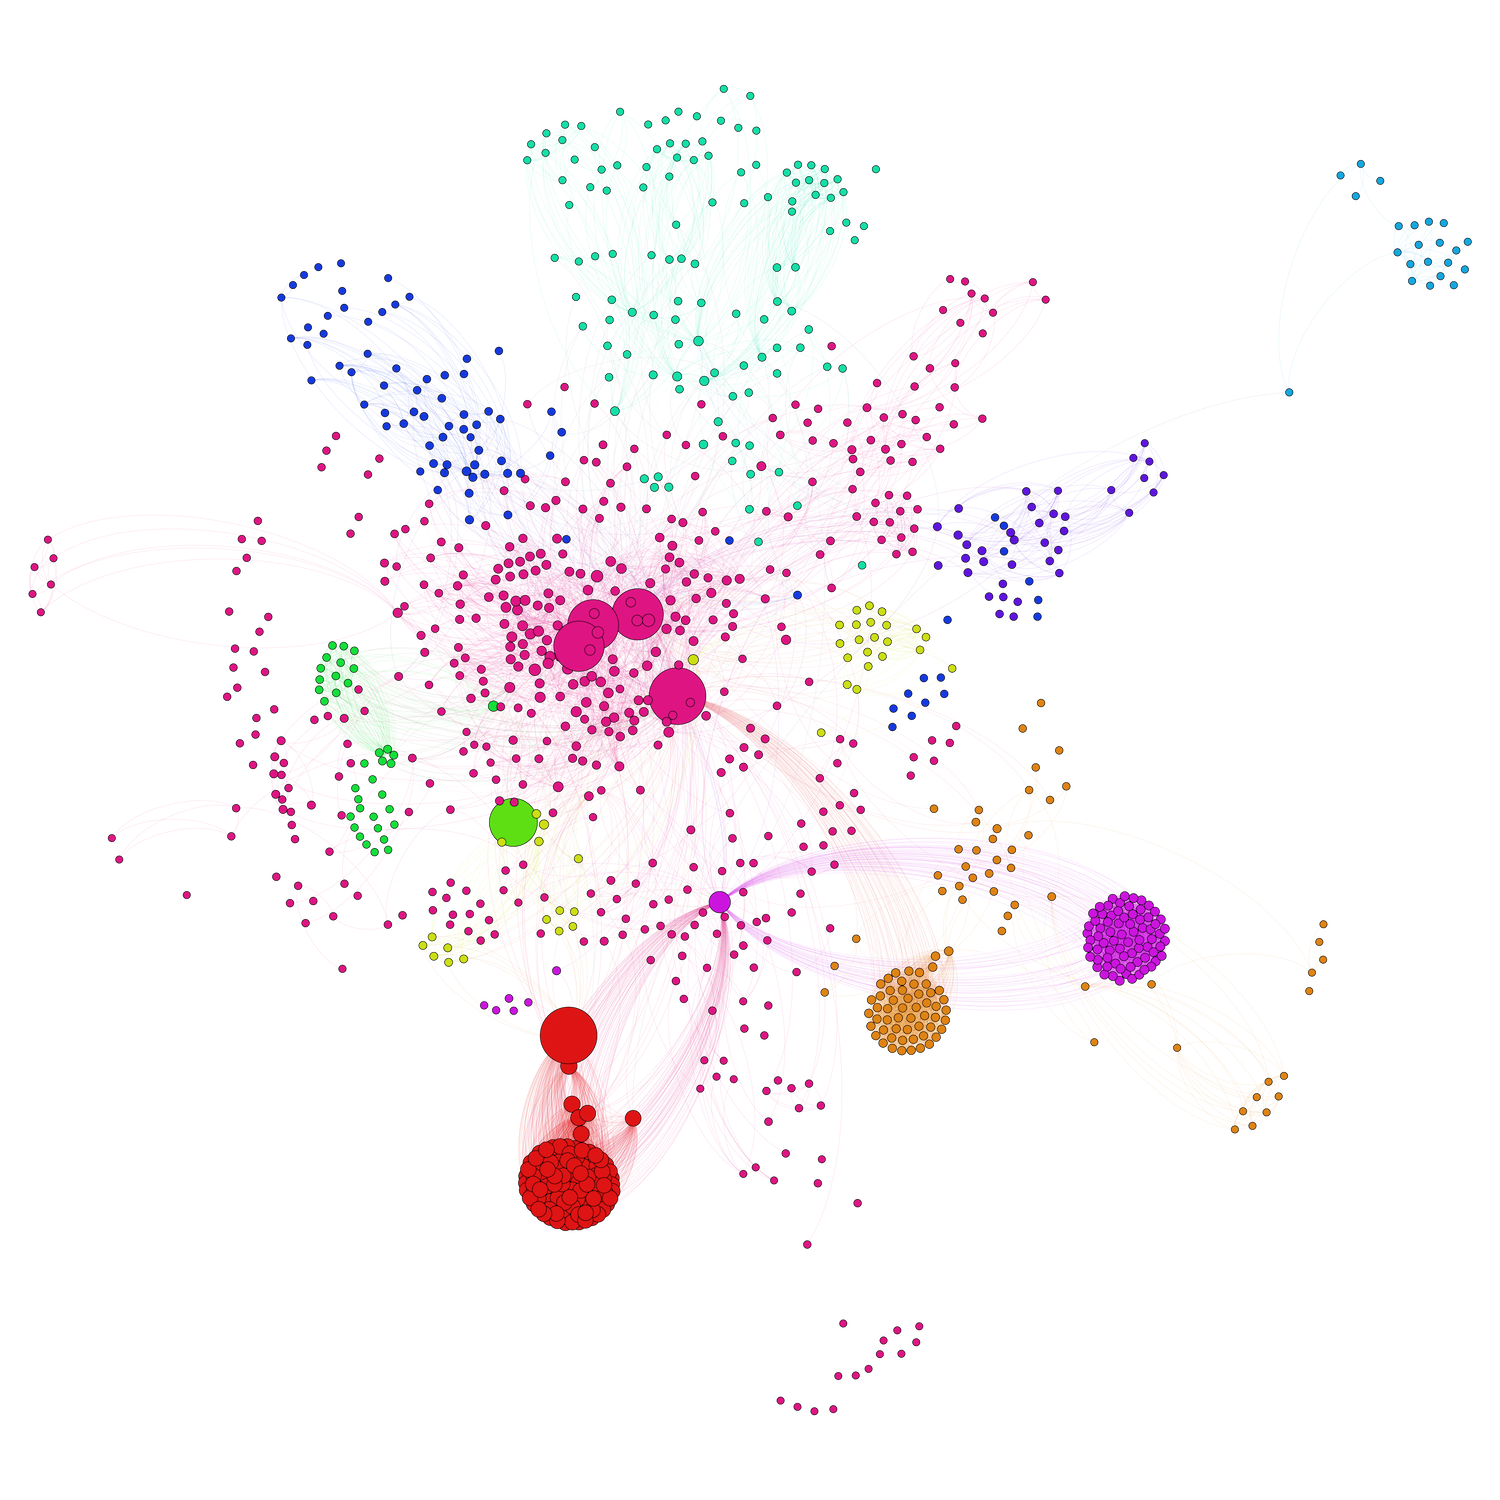
\includegraphics[width=\textwidth]{figures/benjamin_cluster.png}
		\caption{\textsf{Benjamin Bengfort (large)}}
        \label{fig:benjamin_cluster}
	\end{subfigure} \hfill
	\begin{subfigure}{0.49\textwidth}
		\centering
		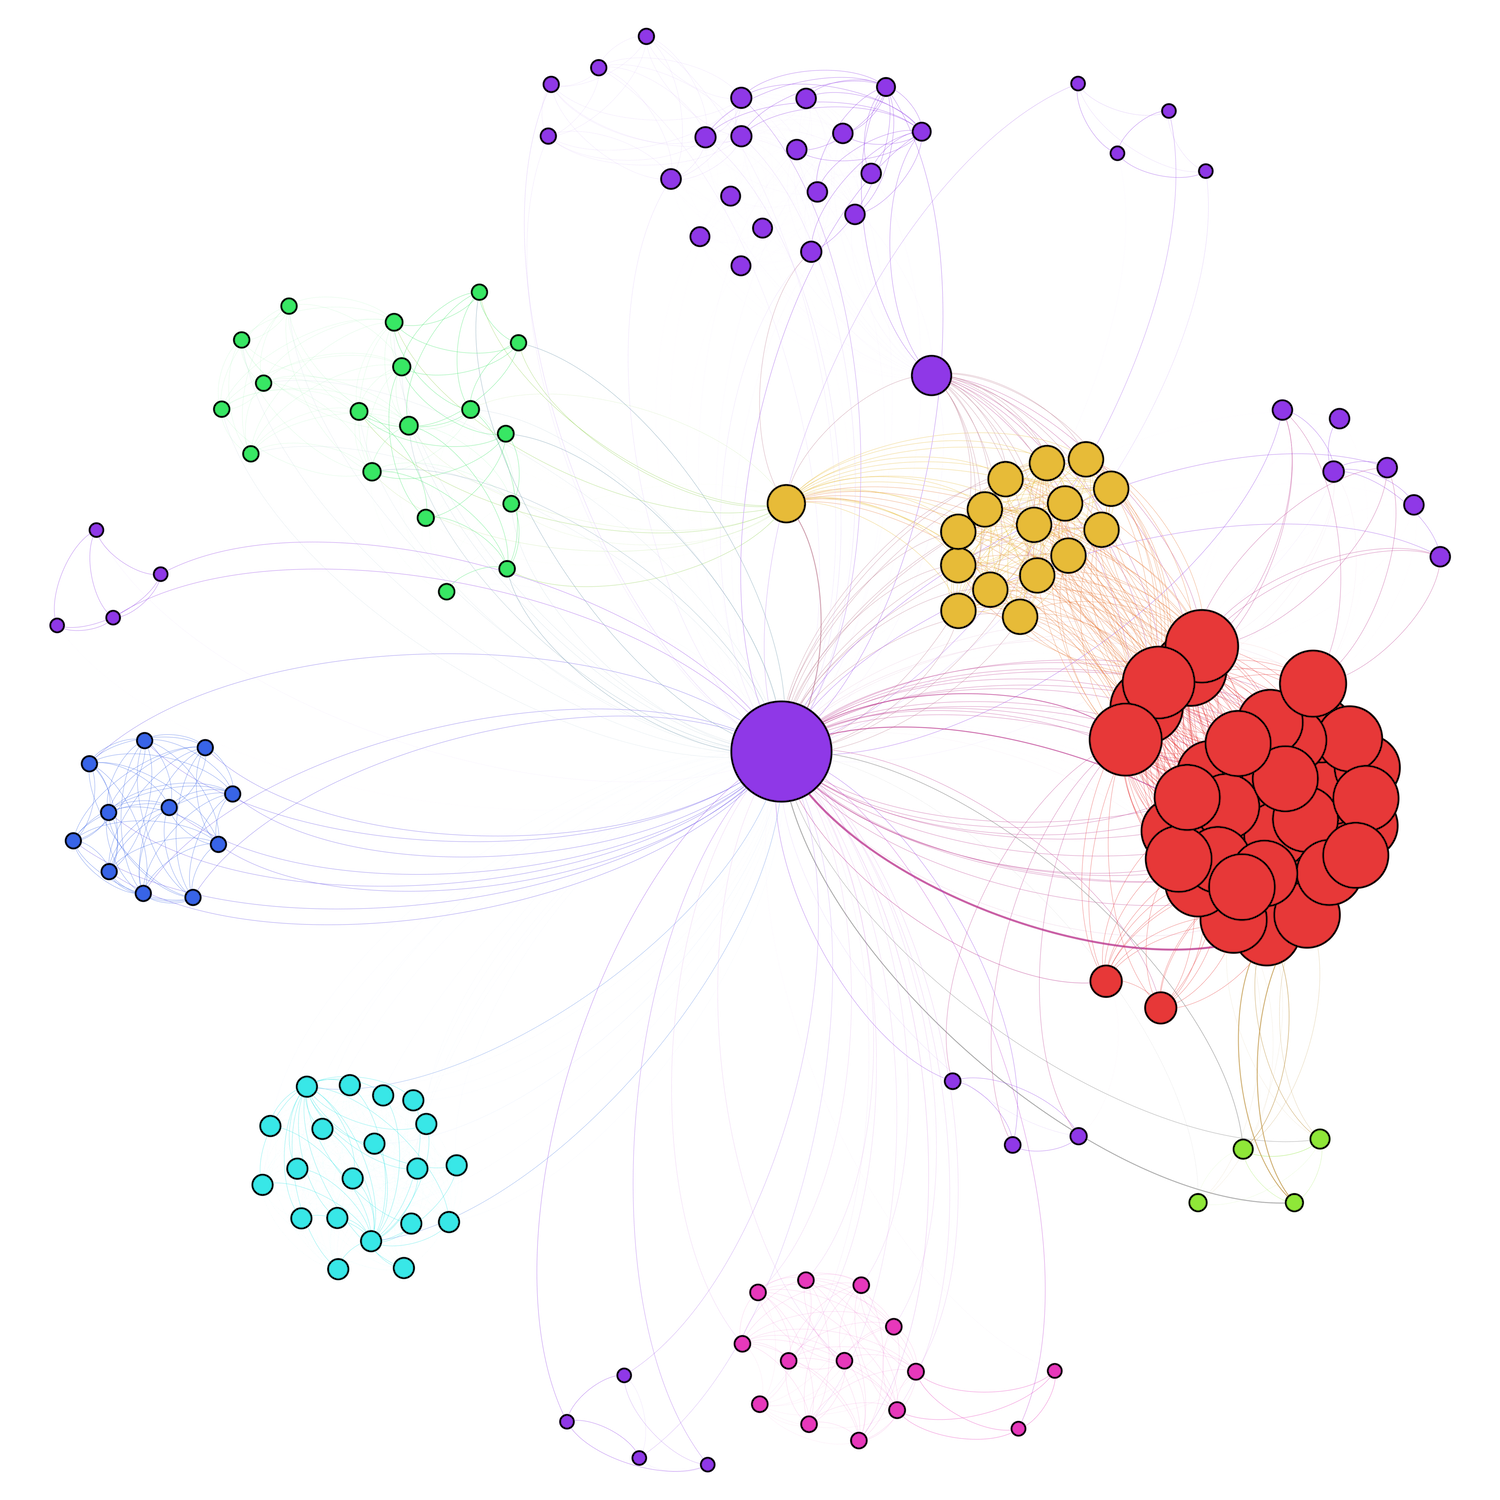
\includegraphics[width=\textwidth]{figures/kostas_cluster.png}
		\caption{\textsf{Konstantinos Xirogiannopoulos (small)}}
        \label{fig:kostas_cluster}
	\end{subfigure}
    \caption{\textsf{Clusters (modularity) colored in email network.}}
    \label{fig:cluster}
\end{figure}

By visualizing our email networks from multiple angles with the help of many useful features that \textit{Gephi} provides, we were able to extract and reason about about clusters that form around the central node. To simplify our cluster analysis we used \textit{K-Core filtering} to remove low degree nodes. To discover clusters, we used the \textit{modularity} feature to partition the graph into highly cohesive groups, visually indicated by color. As seen in \ref{fig:cluster} several clusters are detected, which include the center node, but also others that are disjointed from the core network. Some clusters are loosely connected, while others share very dense sets of connections. By using the Fruchterman Reingold \cite{fruchterman_graph_1991} layout algorithm, the clusters appear very clearly, in an organized fashion around the center node in the ``small'' graph. For the ``large'' graph, we found that the Yifan Hu proportional layout \cite{hu_efficient_2005} made the graph more comprehensible. These layout and statistical algorithms draw the human eye to particular clusters and through further interaction using Gephi we were able to start digging deeper into what they signify.

A first quick observation shows that not all clusters are structurally similar: some are densely connected while others are more sparse, including an ``other'' cluster which seems to contain any node that doesn't belong to a group. For communities where communication is sparse and occasional some cliques do appear, however node degrees are very low (e.g. the blue cluster in ``small'' graph). There also appear extremely large and dense clusters where vast amounts of emails travel back and forth between different nodes in the cluster (e.g. the \textit{red} clusters in both graphs). We believe these types of clusters (of the type seen here) signify collaborative email, where users are \texttt{CC}'d with each other and many different users initiate the conversations.

\section*{Critique}

Gephi has some very significant advantages for visual network analysis. It is a multi-platform tool that can be used for a wide array of graph visualizations. Indeed, one of the most important steps of network visualization is proper layout. Gephi includes few, effective layout algorithms that have been optimized for medium to large networks. One type of visual analysis we discovered was laying out the graph in various ways, and generating insights that were dependent on the size and shape of the resulting network. Gephi also includes a variety of \textit{filtering} features, which allow the user to extract a simplified subgraph, usually one that only includes significant nodes and edges to particular analyses. Finally, Gephi exposes a number of graph statistics, also optimized for medium to large graphs, which can used as parameters in visualization. Overall, we believe that an expert user who is already somewhat familiar with Gephi can easily go from raw graph data to insightful visualizations in a matter of a few minutes. Gephi is not as complete as NodeXL - but scales well in a computationally intensive domain.

Like any tool, however, Gephi has disadvantages as well, and unfortunately in this case they are critical to its usability. First, we found several very severe bugs in Gephi. For instance, when the user saves their progress on a visualization in a \texttt{.gephi} project file, it seems the file cannot then be re-opened. For all our analyses on both graphs we were forced to start from the beginning and re-trace their steps to get the desired result. Gephi does support workspaces, but was very buggy and slowed down considerably with larger graphs. Furthermore, there is no obvious \textbf{undo} functionality in Gephi, nor the typical \texttt{CTRL+Z} keybinding. This lack is unfortunate and makes the tool difficult to use. In interactive analyses it is critical that a user is able to revert changes made in the exploratory and sense-making process. Gephi has a steep learning curve, many iterations are required before the user understands each filter and layout and is able to get her graph down to a manageable size and shape.

From our experience with NodeXL in class, we would say that NodeXL is more feature-rich in terms of interactive analysis than Gephi is. NodeXL is certainly more user focused, whereas Gephi is developer and expert focused, providing a more academic experience. Possibly for this reason, Gephi is prone to simple bugs and frustrations, even while it exposes algorithms that are on the cutting edge of science. However, Gephi is optimized for larger networks than we have seen used in NodeXL; it seems that a dedicated system rather than a tie into Microsoft Excel made it more easily accessible on other platforms.

\section*{Conclusion}

In this paper, we became familiar with and applied the widely-used network visualization tool \textit{Gephi} to explore the inner workings of our email networks. We simplified the networks and found out how ``hubs'' connect different parts within these networks and learned that individuals who act as hubs within our communities are different than the ones we'd identify in day to day networking. Moreover, we identified the key players in our network and which key players act as communication hotspots between the community of people with whom we interact.  We discovered that email contacts central to our communication don't often have a high degree of connectedness to other contacts. We detected sparse and dense clusters within our networks and found that although the communities were well determined (e.g. work, school, and personal communities) not all of our communities share as tight bonds with each other. Finally we critiqued Gephi as an interactive visual analysis tool and compared it to NodeXL.

By exploring our own personal email networks, we hoped to reveal that the communication networks we participate in are more inclusive and demonstrate more about our behavior than our \textit{performed} social networks -- and boy did we! Many of our interactions with the visual aspects of our networks from simplification, sizing and coloring nodes, and aggregating edges revealed surprising players and communities within communities. In the future, we might use such analyses to optimize how we communicate with others, for example by always including ``hubs'' in our correspondence to ensure that news travels more rapidly without the privacy concerns of broadcast media! 

\bibliographystyle{plain}
\bibliography{paper}

\end{document}
